% -*- mode: fundamental -*-

% ****************************************************************

\chapter{BSV: Struct types and tuples; and\\
RISC-V: Memory requests \& responses}

\markboth{Ch \arabic{chapter}: BSV structs; RISC-V mem reqs and rsps}{\copyrightnotice}

\setcounter{page}{1}
% \renewcommand{\thepage}{\arabic{page}}
\renewcommand{\thepage}{\arabic{chapter}-\arabic{page}}

\label{ch_Structs_Mem_Reqs_Rsps}

% ****************************************************************

\section{RISC-V: structs communicated between stages}

\index[BSV]{struct!hetoregeneous collection of values}
\index[BSV]{field!of a {\tt struct}}
\index[BSV]{member!of a {\tt struct}}

In Figure~\ref{Fig_Simple_Instr_Exec_w_structs}, various kinds of
information need to be communicated between the stages---program
counter values, instructions, values read from registers, values to be
written back to registers, and so on.
\begin{figure}[htbp]
  \centerline{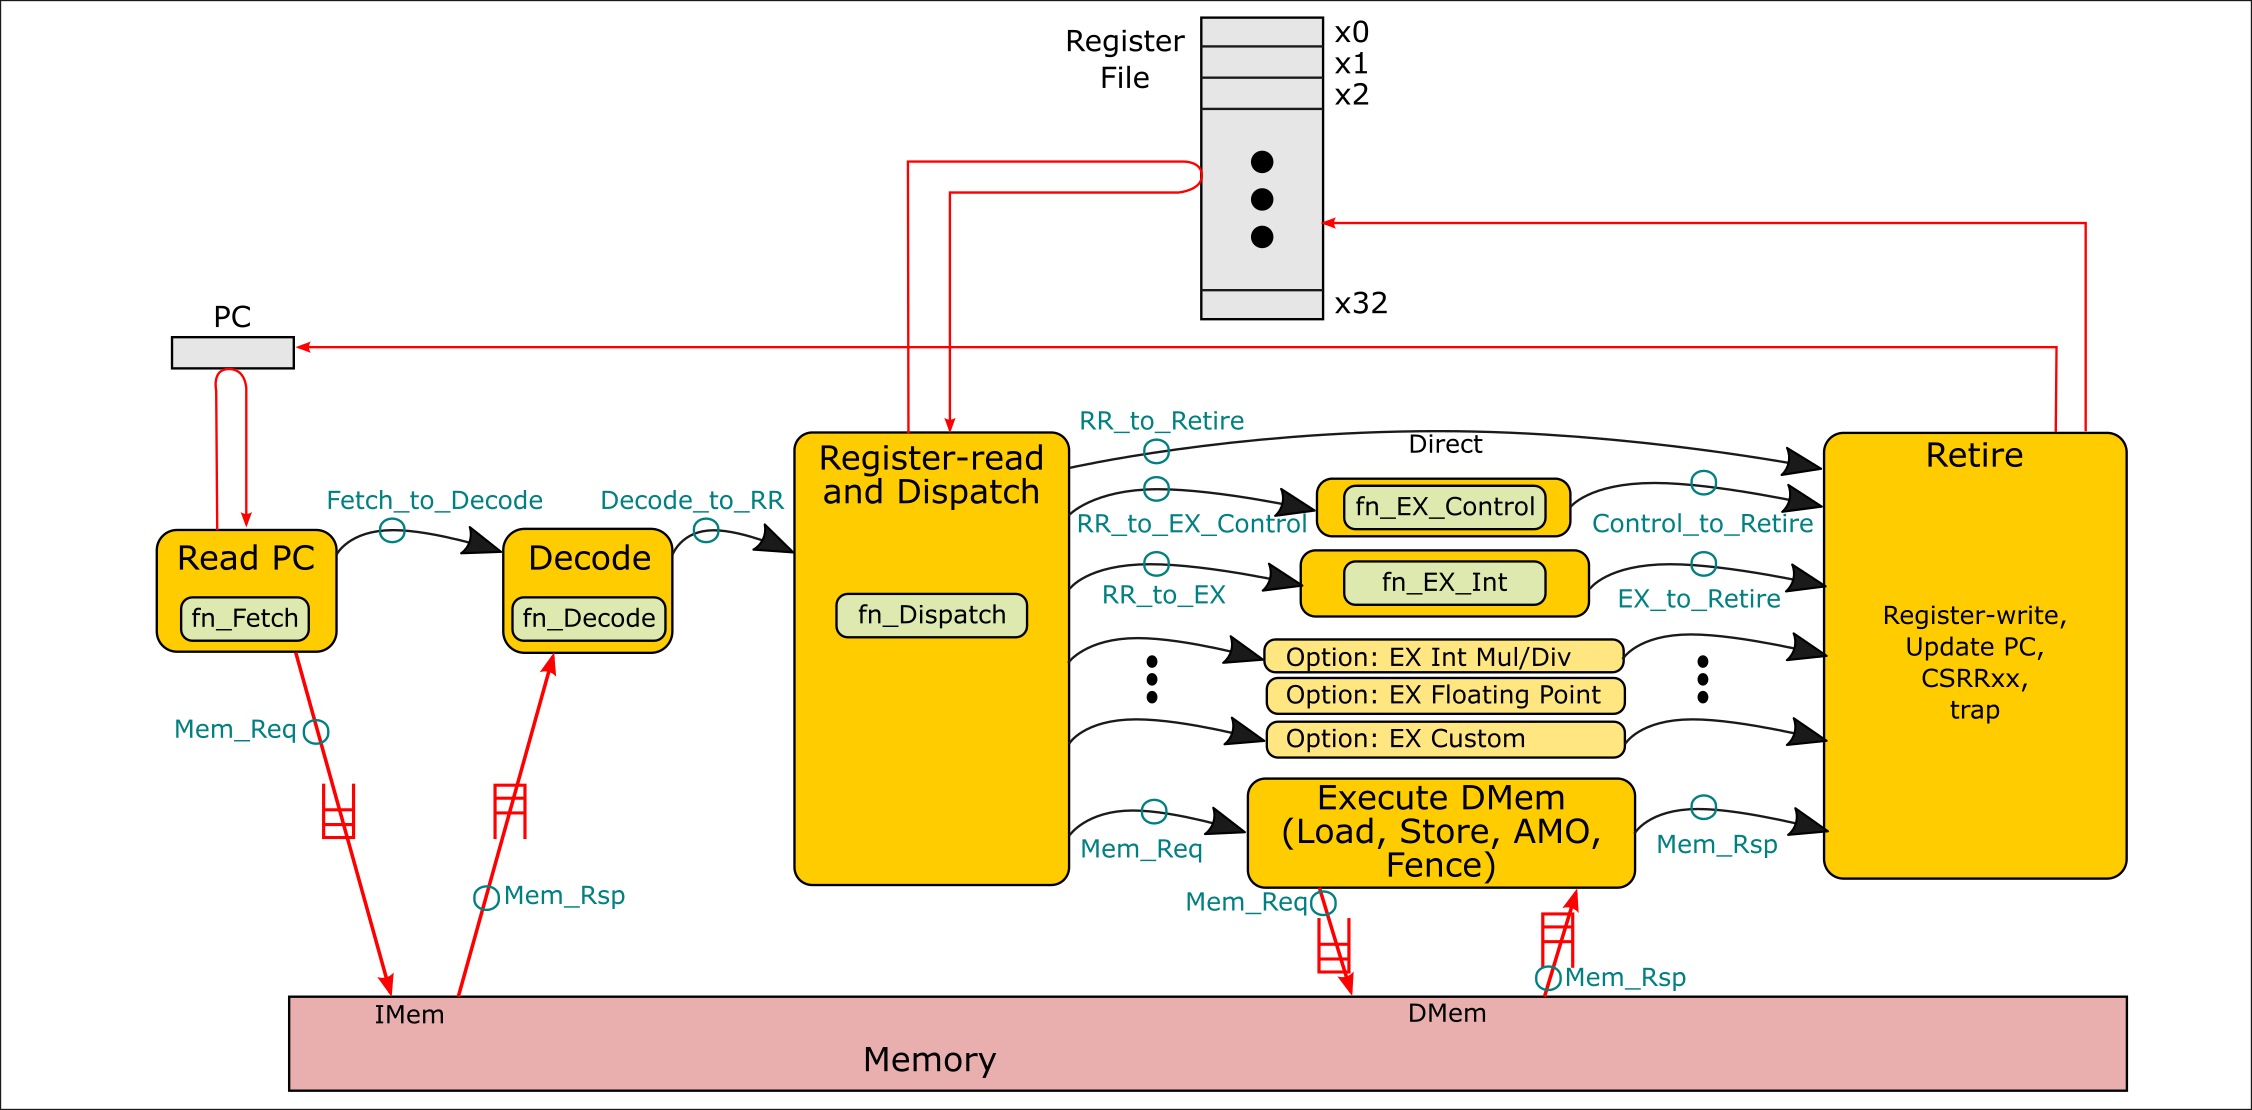
\includegraphics[width=6in,angle=0]{Figures/Fig_Instr_Exec_w_structs}}
  \caption{\label{Fig_Simple_Instr_Exec_w_structs}
           Simple interpretation of RISC-V instructions \\
	   \hmmmm\hmm (Same as Fig.~\ref{Fig_Instr_Exec}, with arrows annotated with {\tt struct} types)}
\end{figure}
\verb|struct| data types (short for ``structures'') are suitable for
bundling together heterogeneous collections of
values.\footnote{Structs in {\BSV} are just like structs in C/C++ and
SystemVerilog.  They are also known as ``records'' in some programming
languages.}  Each component of a struct is called a ``field'' or a
``member'' of the struct.
Figure~\ref{Fig_Simple_Instr_Exec_w_structs} annotates
Figure~\ref{Fig_Instr_Exec} with struct types communicated on each of
the black arrows between stages, and each of the red arrows to and
from memory.  In this and the next few chapters we will flesh out the
details of all these struct types.  We will use exactly the same
struct types for Fife and Drum, {\ie} whether the implementation is
pipelined or not.  All these \verb|struct| declarations can be found
in the file: \verb|src_Common/Inter_Stage.bsv|.

% ****************************************************************

\section{BSV: {\tt struct} types}

\label{BSV_struct_types}
\label{Sec_Mem_Req}

In Figure~\ref{Fig_Simple_Instr_Exec_w_structs}, consider the red
arrow from the Fetch stage to the IMem port of memory, or the red
arrow from the Execute DMem stage to the DMem port of memory.  We want
to communicate several values, including:

\begin{tightlist}
 \item The type of memory request: LOAD, STORE, {\etc}
 \item The size of the memory request: 1, 2 or 4 bytes.
 \item The address in memory that is to be accessed.
 \item For a STORE, the data to be written.
 \item ... (possibly additional fields for debugging) ...
\end{tightlist}

\index[BSV]{struct@{\tt struct}!type declaration}
\index[RV]{Memory!Request}

This heterogeneous collection of values ({\ie} collection of values of
different types) is most conveniently expressed as a \verb|struct|
type:

\SHOWCODE{Code_Extracts/Mem_Req.tex}

Here, we are defining a new type {\tt Mem\_Req} containing fields like
{\tt req\_type}, {\tt size}, {\tt addr} and {\tt data}, each having a
specific type.  We will discuss \verb|Mem_Req_Type| and
\verb|Mem_Req_Size| soon (in Sections~\ref{Sec_Mem_Req_Type} and
\ref{Sec_Mem_Req_Size}, respectively); for now, just think of them as
enum types (small bit-width scalars).

The order in which the fields are declared has no semantic
significance; the order can be chosen freely for best
readability.\footnote{The order of fields will affect the bit-vector
representation of the struct (see
Section~\ref{Sec_struct_representation}) but that is an implementation
detail, not a semantic property.}

% ================================================================

\subsection{Creating (constructing) struct values}

\index[BSV]{struct!entire struct values}

We can create a new value of type \verb|Mem_Req| with syntax like
this:

{\footnotesize
\begin{Verbatim}[frame=single, numbers=left]
   Mem_Req x = Mem_Req {req_type: ... value of field ... ,
                        size:     ... value of field ... ,
                        addr:     ... value of field ... ,
                        data:     ... value of field ... ,
                        ...   };
\end{Verbatim}
}

The identifier {\tt Mem\_Req} is used in two ways.  On the left, as
usual, it is the \emph{type} of the identifier that we are declaring
({\tt x}).  On the right, it is a \emph{constructor}, {\ie} it takes
the field values and constructs a struct value.  The entire right-hand
side is sometimes called a ``struct expression'', {\ie} it is an
expression which, when evaluated, produces a struct value.

% ----------------
\vspace{2ex}

NOTE: \fbox{\small
\begin{minipage}{5in}

In C, we use the term ``value'' only for ``small'' items that are
$\leq 64$ bits in size (integers, floating point values, and
pointers).  This is an unfortunate legacy view perhaps tied to
implementation detail---things that can be passed in registers---which
should not be relevant in the semantics of a high-level language.  In
more modern languages (including C++) we can have values of any size,
including structs, arrays, arrays of structs, and so on.

\end{minipage}}

\vspace{2ex}
% ----------------

The repetition of \verb|Mem_Req| above seems verbose.  The \emph{bsc}
compiler's type-analysis is easily able to infer the type from the
right-hand side, so we can just use the keyword ``\verb|let|'' ({\tt
let}-bindings are discussed in Section~\ref{Sec_let_binding}):

\index[BSV]{let@{\tt let}!binding an identifier with implicit type declaration}

{\footnotesize
\begin{Verbatim}[frame=single, numbers=left]
   let  x   =  Mem_Req {req_type: ... value of field ... ,
                        size:     ... value of field ... ,
                        addr:     ... value of field ... ,
                        data:     ... value of field ... ,
                        ...   };
\end{Verbatim}
}

The order in which the field values are given does not matter.  In
particular, the order may be different from the order in the {\tt
typedef} declaration.  The \emph{bsc} compiler will put the fields
into the correct offsets in the struct value.

Not all field values need be given in a struct expression.  The
\emph{bsc} compiler will issue a warning for each unspecified field,
and insert an ``unspecified'' (and unpredictable) value there.  You
can indicate that a field is intentionally left unspecified (and
suppress the compiler warning) using ``\verb|?|'', {\BSV}'s notation
for a ``don't care'' value (these are discussed in
Section~\ref{Sec_Dont_Care_Values}).

{\footnotesize
\begin{Verbatim}[frame=single, numbers=left]
   let  x   =  Mem_Req {req_type: MEM_REQ_LOAD,
                        size:     ... value of field ... ,
                        addr:     ... value of field ... ,
                        data:     ?,
                        ...   };
\end{Verbatim}
}

In our example, when the \verb|req_type| field is \verb|MEM_REQ_LOAD|
the \verb|data| field is meaningless, and we indicate this explicitly
with ``\verb|?|''.

% ================================================================

\subsection{Selecting struct fields}

\index[BSV]{struct!field selection}

Struct fields can be selected using the usual ``dot'' notation common
to SystemVerilog and C/C++:

{\footnotesize
\begin{Verbatim}[frame=single, numbers=left]
   x.req_type
   x.size
\end{Verbatim}
}

% ================================================================

\subsection{Updating struct fields using assignment}

\index[BSV]{struct!field assignment/update}

Struct fields can be updated with assignment using the usual ``dot''
notation common to SystemVerilog and C/C++:

{\footnotesize
\begin{Verbatim}[frame=single, numbers=left]
   x.req_type = MEM_REQ_STORE;
   x.data     = ... new value ... ;
\end{Verbatim}
}

% ================================================================

\subsection{Representation of a struct in bits}

\label{Sec_struct_representation}

\index[BSV]{deriving!Bits}

Because we said ``\verb|deriving(Bits)|'' in the struct type
declaration, the {\bsc} compiler will automatically work out a
representation in bits for \verb|Mem_Req| struct values, using the
straightforward method of simply concatenating the bit-vector
representation of each field into a wider bit-vector for the whole
struct.  The total bit-size of a \verb|Mem_Req| struct value is simply
the sum of the bit-sizes of the individual fields.

If we had \emph{not} said ``\verb|deriving(Bits)|'', the {\bsc}
compiler will not define any bit-representation for this type.  As
mentioned in Section~\ref{Sec_deriving_Bits}, (a) we do not need any
hardware representation in bits for types that are only used at
statically (at compile time) and (b) if we \emph{do} need a
bit-representation, {\BSV} has a mechanism for specifying this
explicitly (``typeclass instances'').

% ----------------
\vspace{2ex}

NOTE: \fbox{\small
\begin{minipage}{5in}

\index[BSV]{packing of struct fields and vector elements}
\index[BSV]{structs!packing of fields}
\index[BSV]{vectors!packing of fields}

In C/C++, compilers will often ``pad'' out fields (insert unused bytes
between fields) so that fields are aligned on byte and word
boundaries, for more efficient access in byte-structured memories.
Thus, a struct's size in C/C++ may be larger than the sum of the field
sizes, and may even vary depending on the compiler's target
architecture or optimization flags.

\vspace{1ex}

In hardware design, struct values reside on wires, in registers, in
FIFOs, {\etc} which have no ``byte-structured'' bias, and so we do not
play any such ``padding'' games in {\BSV}.

\vspace{1ex}

SystemVerilog makes a distinction beteen ``packed'' and ``unpacked''
values; the former may have padding (for efficient simulation) whereas
the latter has no padding (for efficient hardware).

\end{minipage}}
% ----------------

% ================================================================

\subsection{Printing a struct for logging/debugging}

We can print a struct value directly, {\eg}

{\footnotesize
\begin{Verbatim}[frame=single, numbers=left]
    Mem_Req mem_req;
    ...
    $display ("mem_req is: ", mem_req);
\end{Verbatim}
}

It will simply print a hexadecimal representation of the entire
bit-vector representing {\tt mem\_req}.  This can be quite difficult
to read, for two reasons.  First, the bit-vector representing a struct
can be quite large (sometimes hundreds of bits!).  Second, because
bits are packed, fields may not align with hexadecimal digit
boundaries, and so one cannot correlate hexadecimal digits directly
with fields.  A similar problem arises if we view a struct-valued
signal in a waveform viewer, which does not know anything about {\BSV}
types and just shows the hexadecimal value.

For this reason, experienced {\BSV} coders sometimes (perhaps
temporarily for debugging) rearrange the order and sizes of fields in
a struct so that they are well-aligned with hexadecimal digit
boundaries.

\index[BSV]{deriving!Fshow}

Because we said ``\verb|deriving(FShow)|'' in the type declaration,
the \emph{bsc} compiler will automatically define an
``\verb|fshow()|'' function for this type.  This gives us a way to
print a struct in a more readable format:

{\footnotesize
\begin{Verbatim}[frame=single, numbers=left]
    Mem_Req mem_req;
    ...
    $display ("mem_req is: ", fshow (mem_req));
\end{Verbatim}
}

{\footnotesize
(Note: we described \verb|deriving (FShow)| for enum types in
Section~\ref{Sec_deriving_FShow}).}

Now, the printout will look something like this:

{\footnotesize
\begin{Verbatim}[frame=single, numbers=left]
Mem_Req { req_type: 'h1e, size: MEM_4B, addr: 'h0000000080000000,
          data: 'h0000000000000000, ...}
\end{Verbatim}
}

{\ie} the struct value display is formatted to show the struct type
and the individual fields.

% ================================================================

\subsection{Memory request type}

\label{Sec_Mem_Req_Type}

A memory-request in RV32I is either a LOAD, a STORE or a FENCE.  We
could define an enum type for this:

{\footnotesize
\begin{Verbatim}[frame=single, numbers=left]
typedef enum {MEM_REQ_LOAD,
              MEM_REQ_STORE
              MEM_REQ_FENCE} Mem_Req_Type
deriving (Bits, FShow, Eq);
\end{Verbatim}
}

which will use a 2-bit encoding (0 for LOAD, 1 for STORE, 2 for
FENCE).  However, we look to the future where we might extend Drum and
Fife to implement the ``A'' extension (for AMO or ``Atomic Memory
Operations'').  The RISC-V ISA Unprivileged Spec document, Chapter 8,
describes additional memory operations LR (Load-Reserved), SC
(Store-Conditional), AMOSWAP, AMOADD, AMOXOR, AMOAND, AMOOR, AMOMIN,
AMOMAX, AMOMINU, and AMOMAXU, each of which comes in a 32-bit version
(in RV32 and RV64) and a 64-bit version (in RV64).  These operations
are coded with 5 bits in the instruction (\verb|instr[31:27]|, which
we call ``{\tt funct5}'').

Accordingly, we use a 5-bit encoding for the memory request type.
When we implement the A extension, we will directly use the 5-bit
codes from the instruction.  For LOAD, STORE and FENCE we use 5-bit
codes that are unused in the A extension:

\SHOWCODE{Code_Extracts/funct5_MEMOPs.tex}

% ================================================================

\subsection{Memory request size}

\label{Sec_Mem_Req_Size}

An IMem request is for one 32-bit instruction (4 bytes).\footnote{When
implementing the ``C'' RISC-V ISA extension (compressed instructions),
instructions can also be 16-bits (2 bytes).  When implementing more
sophisticated Fetch units, we may actually fetch chunks larger than 4
bytes, such as a full cache line.}

An RV32I DMem request may be for 1, 2 or 4 bytes.  Looking to the
future, accesses may also be for 8 bytes (doublewords in RV64I, and/or
double-precision floating point values in the ``D'' ISA extension for
RV32 and RV64).  We express these request-size options using an enum
type:

\SHOWCODE{Code_Extracts/Mem_Req_Size.tex}

Similarly, we have also declared the \verb|addr| and \verb|data|
fields in the \verb|Mem_Req| struct to be 64 bits, not 32.  For STORE
requests of 1 and 2 bytes ({\ie} smaller than the \verb|data| field)
we assume the data is passed in the least-significant bytes of the
\verb|data| field.

% ****************************************************************

\section{BSV: Tuples and the {\tt match} statement}

\label{Sec_Tuples}

\index[BSV]{Tuples}

Tuples are a special kind of pre-defined \emph{immutable} structs in
{\BSV}.\footnote{
Python has a similar concept of immutable tuples, and pattern-matching
to access tuple components.
}
For example, when a function needs to return a pair of values, instead
of declaring a struct type with two fields for the result, it is often
more convenient to just use the built-in \verb|Tuple2| type.  Example:

{\footnotesize
\begin{Verbatim}[frame=single, numbers=left, label=in src\_Common/CSRs.bsv]
   function ActionValue #(Tuple2 #(Bool, Bit #(XLEN)))
            fav_csr_read (Bit #(12) csr_addr);
      ...
	 return tuple2 (exception, y);
   endfunction
\end{Verbatim}
}

The function returns a pair of values which have types \verb|Bool| and
\verb|Bit#(XLEN)|, respectively.  The overall type of the result is
\verb|Tuple2 #(Bool, Bit #(XLEN))|.

The expression in the \verb|return| statement shows how one can
construct a 2-tuple value: simply apply the predefined function
\verb|tuple2| to the two component values.

Tuples are special in {\BSV} because, unlike structs, tuples are
immutable---there is no assignment statement to update a field of a
tuple.

Tuples are also special in {\BSV} because there is no ``.field''
notation for component selection.  To select an individual field of a
tuple, one can use one of the built-in selector functions:

{\footnotesize
\begin{Verbatim}[frame=single, numbers=left]
   let xy <- fav_csr_read (...);
   let exc = tpl_1 (xy);    // exc has type: Bool
   let v   = tpl_2 (xy);    // v   has type: Bit #(XLEN)
\end{Verbatim}
}

Alternatively, to access multiple fields of a tuple at once, one can
use a ``match'' statement. Example (from \verb|src_Drum/CPU_FSM.bsv|):

\index[BSV]{Tuples|match@{\tt match} statement (pattern-matching_)}
\index[BSV]{Pattern matching!match@{\tt match} statement for tuples}

{\footnotesize
\begin{Verbatim}[frame=single, numbers=left]
   match { .exc, .v } <- fav_csr_read (csr_addr);
\end{Verbatim}
}

The \verb|match| keyword is followed by a \emph{pattern} that should
match the tuple, {\ie} here it should be a list of two variable names
surrounded by braces with each variable preceded by a ``\verb|.|''.
The leading ``\verb|.|'' is important: ``\verb|x|'' would represent
the value of an existing variable to be matched with the corresponding
value in the tuple, whereas ``\verb|.x|'' \emph{introduces a new
variable} \verb|x| to be bound to the corresponding value in the
tuple; the latter is what we want.  We refer the reader to the {\BSV}
Language Reference Guide~\cite{BSV_Lang_Ref_Guide} for many more
capabilities of pattern-matching, including fields to be ignored,
pattern-matching on structs and tagged unions, pattern-matching
\verb|case| expressions, and more.

{\BSV} defines tuples of up to 8 components ({\tt Tuple\_3}, {\tt
Tuple\_4}, ...) but we recommend not using tuples when you have more
than, say, 2 or 3 components; define a struct instead, with readable
and meaningful field names.

% ****************************************************************

\section{RISC-V: Memory Requests and Responses; IMem and DMem}

\index[RV]{IMem| Instruction Memory}
\index[RV]{DMem| Data Memory}
\index[RV]{IMem (instruction memory)}
\index[RV]{DMem (data memory)}

In Figure~\ref{Fig_Simple_Instr_Exec_w_structs}, the \verb|Mem_Req|
and \verb|Mem_Rsp| structs are used in two places.  The Fetch stage
issues a memory request, and the corresponding memory response is
received by the Decode stage.  Similarly, the ``Execute Memory Ops''
stage issues a memory request and consumes a memory response.  We use
the shorthand term ``IMem'' for the first context (for Instruction
Memory) and ``DMem'' for the latter context (for Data Memory).

% ================================================================

\subsection{Separation of IMem and DMem (Harvard Architecture)}

\label{Sec_Harvard_architecture}

\index[RV]{Harvard architecture}
\index[RV]{Harvard architecture!Self-modifying code}

The separation of memory channels for instructions and data
(loads/stores) is quite standard in modern CPU architectures, and is
informally called a ``Harvard Architecture''.  The term refers to the
architecture of the Harvard Mark I computer, designed and built by
Harvard University and IBM in the 1940s (the term itself was coined
much later).  It sometimes refers just to separate, concurrent paths
to memory for instructions and data, and sometimes also to physically
separate memories for instructions and data (more discussion in
Wikipedia:~\url{https://en.wikipedia.org/wiki/Harvard_architecture}).

Modern software is typically not ``self-modifying'', {\ie}
instructions and data are placed in different areas of memory, and
load/store instructions never write into the instruction area, {\ie}
programs never over-write instructions in memory.  This allows
separate hardware for memory access for instructions {\vs} memory
access for data, which can run concurrently, {\ie} we may fetch an
instruction at the same time as we are accessing data memory for a
previous load/store instruction (we will see this in Fife).  We can
also tune and optimize each memory path separately for their different
dynamic behavioral patterns.  In some systems we can also
\emph{protect} the instruction memory area, {\ie} enforce in hardware
the policy of not over-writing instructions.

\index[RV]{JIT (Just-in-time compiling)}
\index[RV]{Just-in-time compiling (JIT)}

This view of strict separation of IMem and DMem has to be tempered
somewhat when considering languages like JavaScript, Python {\etc}
that employ so-called ``JIT'' compiling (``Just-In-Time'').  The
run-time systems of such languages generate instructions on-the-fly,
{\ie}, LOAD/STORE instructions produce \emph{data} through the DMem
channel that will (soon) be fetched as \emph{instructions}.  But even
in these systems, there is a strict protocol of \emph{phases}.  During
a code-generation phase, the data produced is considered as ordinary
data.  Then there is a deliberately executed phase-change, where the
virtual memory protections of the data-pages just written are changed
so that they are now viewed as read-only instruction pages, after
which these new instructions can be fetched.

% ================================================================

\subsection{Address Alignment}

\index[RV]{Address alignment}
\index[RV]{Memory!Address alignment}

Although nowadays we think of all computer memories in units of 8-bit
bytes and being byte-addressed,\footnote{Some early computers, until
about the late 1970s, had other memory granularities---multiples of 6,
7, 9 bits, {\etc} Those were the days of bespoke memories for each
computer design.  Mass-production of memory chips resulted in
standardization to 8-bit bytes.} in practice in hardware, it is
usually simpler if memory-requests are \emph{aligned} to an address
according to the request size.  Specifically, the address for a 2-byte
request should be even, {\ie} the least significant bit of the
address, \verb|addr[0]|, should be zero.  The address for a 4-byte
request should have zero in the two least significant bits
(\verb|addr[1:0]|) and the address for an 8-byte request should have
zero in the three least significant bits (\verb|addr[2:0]|).

We can see why address-alignment is desirable.  Memory implementations
(chips) are usually architected to retrieve multiple bytes at a time
({\eg} 64 bytes) so that all those bytes can share addressing and
control circuitry.  With such an organization, a misaligned access
request may straddle the boundaries of such ``naturally sized'' units
and so may require two consecutive reads/writes.  Caches are usually
organized to hold multi-byte \emph{cache lines} ({\eg}, 32 bytes) in
order to share the addressing and miss-handling circuitry, and to move
data efficiently in and out of the cache.  Again, a misaligned access
request may straddle a cache-line boundary, and may require two
consecutive accesses, which may hit or miss independently.  Virtual
memory systems are usually organized in \emph{pages}, units of
typically 4K-8K bytes, in order to share virtual-memory handling
circuitry, and to move data efficiently between main memory and disks.
Again, a misaligned access may straddle a page boundary, and may
require two consecutive accesses, which may hit or page-fault
independently and differently.  In short, misaligned accesses add
significant complexity to memory-system hardware design.

We can organize our software so that misaligned accesses are
exceedingly rare.  Most software is produced by compilers, and the
compiler ensures that instructions and data are placed in memory at
aligned addresses, possibly by padding gaps between ``adjacent''
smaller-sized data (such as a pair of 1-byte-sized fields in a
struct).  This padding may waste a few bytes of memory, but pays back
in greater speed and reduced complexity.

Although misaligned accesses are rare, we cannot always guarantee
their absence in software, since software can calculate an arbitrary
address before performing a memory access.  It seems wasteful to have
to pay for extra hardware complexity (with attendant loss in overall
performance) for such rare cases.  In many computer systems,
therefore, these rare misaligned accesses are relegated to software
handling:

\begin{tightlist}

\item The memory system simply refuses to handle a misaligned access,
  and returns a ``misaligned'' error instead.

\item The CPU, receiving such an error response, undergoes a ``trap''
  which directs it to piece of software called an trap-handler (or
  exception handler).  The trap-handler (in software) performs the
  memory access in multiple smaller pieces (in the worst case, of size
  1 byte), each of which is aligned.  In other words, the trap-handler
  ``completes'' the original memory access before resuming the
  main-line code that attempted it.

\end{tightlist}

The RISC-V ISA specification does not forbid misaligned accesses nor
prescribe how they should be handled.  Some implementations will
handle it in hardware, and other implementations will return a
``misaligned'' error and rely on a trap handler to complete the
access.  Some implementations may only run software where it has been
proven to not generate misaligned memory requests, and therefore may
not even contain a trap-handler for misaligned accesses.

% ----------------------------------------------------------------
\Beginexercise

Please see directory: \hm {\tt Exercises/Ex\_05\_A\_Structs/} \\
and its README.
\Endexercise

% ================================================================

\subsection{Memory Responses}

\label{Sec_Mem_Rsp}

\index[RV]{Memory!Response}

The response from memory for any request may be to report success, an
alignment error, or some other error.  Examples of ``other errors''
are:

\begin{itemize}

\item Absence of memory at the given address.  For example, although
  RV32I addresses are 32-bits, which can address 4GiB of memory, we
  may provision our system with something smaller, say 1 GiB.

\item An unsupported operation. {\Eg} an attempt to write into a
  read-only memory (ROM).

\item Corruption of data, due to electrical glitches, environmental
  electromagnetic pulses, {\etc}.  These errors are usually detected
  with some kind of error-detecting code, such as parity bits.

\end{itemize}

These different memory response-types can be encoded in an enum type:

\SHOWCODE{Code_Extracts/Mem_Rsp_Type.tex}

A memory-response contains the response-type. For a LOAD request with
an OK response, it also contains the data that was read from memory.
This can be expressed in a struct:

\SHOWCODE{Code_Extracts/Mem_Rsp.tex}

For LOAD requests of 1 and 2 bytes ({\ie} smaller than the \verb|data|
field) we assume the data is returned in the least-significant bytes
of the \verb|data| field.

% ----------------------------------------------------------------
\Beginexercise

Please see directory: \hm {\tt Exercises/Ex\_05\_B\_Mem\_Req\_Rsp/} \\
and its README.
\Endexercise

% ****************************************************************
